\chapter{Methodology}
\ifpdf
    \graphicspath{{Chapter2/Chapter2Figs/PNG/}{Chapter2/Chapter2Figs/PDF/}{Chapter2/Chapter2Figs/}}
\else
    \graphicspath{{Chapter2/Chapter2Figs/EPS/}{Chapter2/Chapter2Figs/}}
\fi

\section{Baseline Method}

\begin{figure}[!htbp]
  \begin{center}
    \leavevmode
    \ifpdf
      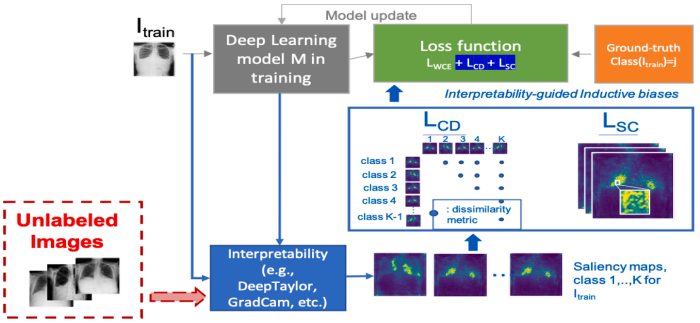
\includegraphics[scale=0.75]
      {Chapter2/Chapter2Figs/sibnet_arch.png}    
    \fi
    \caption{Sibnet Architecture}
    \label{sibnet_arch}
  \end{center}
\end{figure}

We now detail the idea proposed by \cite{MAHAPATRA2022102551} in the paper titled "Interpretability Guided Inductive Bias for Deep Learning Based Medical Image". This is the paper we started out with to reproduce the results of.

The paper takes inspiration from the observation that when a radiologist is performing diagnosis on medical images, they look for disease-specific image patterns or characteristics. We attempt to help the model imitate the same by integrating a novel inductive bias in the loss term of the model along with cross entropy loss such that the learned features yield more class distinctive and spatially coherent saliency maps which makes it easier for the radiologist to diagnose. The bias term we define acts directly on the loss function of the model being trained, it is modular and easy to implement, and can be used in combination with any other loss functions, as well as on existing classification model architectures without any modifications

Figure \ref{sibnet_arch} shows the main pipeline of the approach. A model is trained with a combination of standard classification loss terms and the proposed interpretability-guided inductive bias loss terms. The learned features obtained from the model generate more class distinctive and spatially coherent saliency maps. This makes the learned features of a class as unique as possible from features of other classes and that improves the model performance. Moreover, it enforces an enhanced spatial attention to the class label describing the targeted disease. This helps the radiologist a lot in understanding which regions of an x-ray image describe a particular disease and makes the diagnosis easier. Any deep learning model can be used with our proposed loss term. The paper uses DenseNet121 as it has performed well on medical images classification and it has skip connections which eliminates the problem of vanishing gradients. It is very crucial that we don’t face vanishing gradients problem for this specific task as we use gradients to generate saliency maps.

A saliency map \textbf{$S_{\{I,c\}} \in R^d$}
identifies important regions of an image I which are to
be classified as label c for a given training image I and model M. The proposed
inductive bias aggravates the distinctiveness between saliency maps \textbf{$S_{\{I,c=i\}}$} and \textbf{$S_{\{I,c=j\}} (j \ne i) (\forall i, j \in \{1, ...., K\})$} for different classes of an image I and improves spatial coherence to effectively identify the features of an image used by the model
to perform classification. Two loss terms were proposed to handle separate aspects of multi-class classification.

\subsection{Class distinctiveness Loss}

Given training image $I$ and model $M$, we generate a set of saliency maps $\left\{S_{I, c}\right\}_{c=1}^{K}$ which encodes the explanation for each class $c$. Then, we compute the corresponding latent representations of the saliency maps $\left\{Z_{S_{I, c}}\right\}_{c=1}^{K}$ from the last convolutional layer of the model. The latent representation vectors $Z$ encode the current understanding of the model $M$ to the generated saliency maps.

In order to induce distinctiveness of saliency maps of an image among different classes, we calculate the loss term $\left(L_{C D}\right)$, as follows:

\begin{center}
{ $L_{C D}=\frac{2}{K(K-1)} \sum_{c_{1}=1}^{K-1} \sum_{c_{2}=c_{1}+1}^{K}$ cosine\_similarity $\left(Z_{S_{l, c_{1}}}, Z_{S_{I, c_{2}}}\right)$}
\end{center}


In the above equation, cosine\_similarity(.) is the cosine similarity metric that computer dissimilarity of 2 vectors where 1 denotes minimum dissimilarity and  0 denotes maximum dissimilarity. We take the average of cosine similarity of all possible pairs of latent representations for an image. The basic intuition make the latent representations $Z$ as dissimilar as possible from each other. Any other similarity metric can be used instead of cosine similarity. As the model training minimizes the loss function, the model eventually learns to minimize the similarity among different latent representations for an image. 

\subsection{Spatial coherence loss}

The objective of the spatial coherence loss term is to regularize the spatial distribution of saliency maps. This function aims to reduce the dispersion of features of saliency maps by making the features as cohesive as possible as that would be closer to the regions annotates by experts and makes it easier for doctors to identify the region of interests with more certainty and perform diagnosis. We propose a spatial coherence loss term $\left(L_{S C}\right.$ ), as follows:

\begin{center}
{$L_{S C}=\sum_{p} \sum_{n_{p} \in \mathscr{T}(p)}\left\|x_{p}-x_{n_{p}}\right\|^{2}$}
\end{center}

In the above equation, $x_{p}$ is the pixel intensity in saliency map $S_{I, c}$ and $x_{n_{p}}$ is the set of pixels in the $9 \times 9$ neighborhood $\mathscr{N}(p)$ belonging to the same cluster as p. 
A small neighbourhood may not provide adequate information about the local neighbourhood whereas the computational complexity is too much for large neighborhood. $9 \times 9$ neighborhood was able to achieve good accuracy with decent computational complexity. Clusters on each saliency map are identified by performing connected component analysis. This loss term penalises the difference in intensity between pixels belonging to same cluster located in a neighborhood and thus ensures that the pixels of same cluster in a neighborhood have similar intensity values making them more spatially coherent.

The total loss is defined as: 
$L_{\text {Total }}=L_{W C E}+\lambda_{1} L_{C D}+\lambda_{2} L_{S C}$ where
$\lambda_{1}$ and $\lambda_{2}$ are the parameters that determine the contribution of class distinctiveness and spatial coherence loss respectively to the loss function.

\section{GradCAM}
GradCAM is a technique to generate saliency maps mainly for Convolutional Neural Networks. There can be various methods to obtain saliency maps as explained in Chapter \ref{chap:litreview}. In our project we have mainly used the Gradient Weighted Class Activation Mapping (GradCAM) \cite{selvaraju2017grad}.
It uses the gradients flowing to the final convolutional layer over any target to produce a coarse localization maps highlighting the important regions used to predict the target.\\
\begin{figure}[!htbp]
  \begin{center}
    \leavevmode
    \ifpdf
      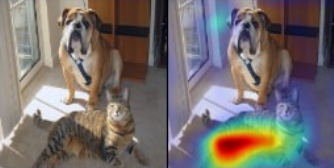
\includegraphics[scale=1]
      {Chapter2/Chapter2Figs/gradcam.png}    
    \fi
    \caption{GradCAM Saliency Map Visualization for "tiger cat" category for VGG16 network, \cite{selvaraju2017grad}}
    \label{gradcam_eg}
  \end{center}
\end{figure}

The gradients of the target class's score with respect to the final convolutional layer of the CNN are calculated by backpropagating the gradients from the output layer to the final convolutional layer, considering only the target class's score and ignoring the other classes. These gradients represent the importance of each channel in the final CNN layer. To quantify the importance of each channel, he activation maps are then averaged over the whole channel. These weights are then finally used to weigh the activation maps across different channels and combine them. ReLu Activation is applied at the end to obtain only non-negative contributions.

Finally the final feature map obtained may be in size smaller than input image. To overcome this the feature map is upsampled using techniques like \textbf{Bilinear Interpolation}.


\section{Modified Pipeline}

\begin{figure}[!htbp]
  \begin{center}
    \leavevmode
    \ifpdf
      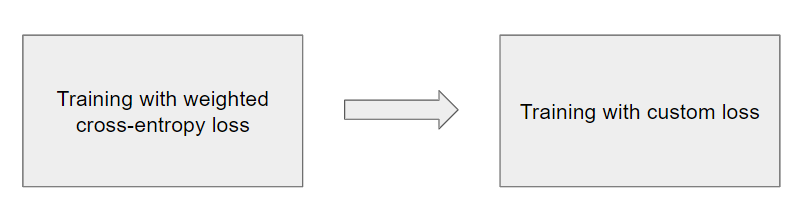
\includegraphics[scale=0.85]
      {Chapter2/Chapter2Figs/modified_pipeline.png}    
    \fi
    \caption{Modified Pipeline}
    \label{mod_pipe}
  \end{center}
\end{figure}

In the given baseline method, the model is trained on the proposed loss functions from scratch. This means that the model starts learning from the pre trained weights as we use pre trained weights of the given architecture. Since both Class Distinctiveness Loss and Spatial Coherence Loss rely on saliency maps, it is important that the saliency maps generated are of adequate quality which means that the saliency maps contain relevant information to help the model better. However, the saliency maps generated in the beginning will not have any information about the location of the object(disease in this case) as the models were pre trained on natural domain images and have no information regarding medical images. Therefore, the initially generated saliency maps may mislead the model and the model may not achieve the desired convergence.

In order to overcome this issue, we propose a modified pipeline of training the model. Figure \ref{mod_pipe} shows the pipeline we have proposed. First we train our model using weighted cross entropy loss only. Once this is done, the model would have learnt the features of the diseases well which leads to better quality of saliency maps with relevant information about the location of the disease learnt by the model. Then, we train our model using the custom loss function. Now, the proposed loss functions will leverage the good quality information provided by the saliency maps to achieve even better performance and saliency maps. Once the training of modified pipeline is done, we can expect to achieve more class distinctive and spatially coherent saliency maps and increase in performance of the model than when compared to training the model on just the custom loss function.  

\section{Loss Functions to address Class Imbalance}

There were few issues with the loss functions proposed in the baseline method. The first issue was that the model training was at least 4 times slower with the custom loss functions than with just cross entropy loss. We attribute this poor performance to the computational complexity of calculating saliency maps. We performed a small experiment where we just fed random data instead of generating saliency maps and then feeding them. We observed that there was no difference in training time between custom loss and cross entropy loss when saliency maps are not generated. Thus, we concluded that generating saliency maps was computationally expensive and there is a need to trade-off between model training time and model performance.

The second issue was that the model performance didn't improve with the custom loss function. The model performance was actually worse with the custom loss functions. Although we were able to close the gap with our modified pipeline, the two proposed loss functions essentially didn't improve the model performance over the standard cross entropy loss function. We concluded that we couldn't improve the performance of the model with the help of performance. We couldn't compare the quality of saliency maps generated by models trained with different loss functions as we neither have the ground truth label of the disease nor the domain expertise to analyse the saliency maps. 

Therefore, we decided to solve a slightly different problem that arises in multi-label medical classification models rather than interpretability. We investigated the class imbalance problem. We found that when the model is trained with weighted cross entropy, there was a huge gap in performance between different classes. For instance, we obtained an AUC of 0.867 for Atelectasis, whereas we obtained an AUC of just 0.691 for Edema. Therefore, we incorporated two new loss functions to address class imbalance problem named Focal Loss introduced by \cite{lin2017focal} and Deep AUC Maximization proposed by \cite{yuan2021large}.

\subsection{Focal Loss}

Focal Loss was first introduced to mainly solve the class imbalance problem in the context of object detection. They discovered that the extreme foreground-background class imbalance encountered
during training of dense detectors is the central cause. They address this class imbalance by reshaping the
standard cross entropy loss such that it down-weights the
loss assigned to well-classified examples. Focal Loss focuses on ensuring predictions improve over hard examples rather than becoming overconfident with easy cases.

It is a dynamically scaled cross entropy loss, where the scaling factor decays to zero as confidence in the correct class increases. Intuitively, this scaling factor can automatically down-weight the contribution of easy examples during training and rapidly focus the model on hard examples. The Focal Loss adds a factor $(1-p_t)^\gamma$ to the standard cross entropy criterion. Setting $\gamma>0$
 reduces the relative loss for well-classified examples $(p_t>0.5)$, putting more focus on hard, misclassified examples. There is a tunable focusing parameter $\gamma\geq0$. 

 Although it was introduced initially to solve class imbalance problem in object detection of objects from natural domain, focal loss has also been used in medical image classification problems down the line \cite{lotfy2019investigation} \cite{tran2019improving} and showed good performance in such settings. This gave us the confidence to go ahead with focal loss. We essentially replace cross entropy loss with focal loss. Focal loss is formally defined as:

 \begin{center}
{ $L_{focal}=-\sum_{i=1}^{i=n}(1-p_i)^{\gamma}log(p_i)$}
\end{center}


\subsection{Deep AUC Maximization}
Deep AUC Maximization is a paradigm to learn deep learning networks with the objective of maximizing the area under the ROC curve, the AUC. Unlike other loss functions mentioned above, DAM directly aims to optimize the AUC rather than minimizing the loss like cross entropy loss.

According to \cite{yuan2021large}, as in medical classification tasks AUC is already the default metric for performance measure during training or evaluating, directly maximizing it helps to increase performance fastest.
Secondly, it is helpful to the medical imaging setting due to the class imbalance nature of datasets, owing to anomalies appearing less often. This is because AUC is more suitable to handle imbalanced data distribution, since maximizing AUC aims to rank score of any positive data higher than any negative data.

AUC according to Wilcoxon-Mann-Whitney statistic is defined as:
\begin{center}
{\textbf{$AUC(w) = Pr(h_w(x) \geq h_w(x')|y = 1, y' = -1)$}}
\end{center}
Above simplifies to, 
\begin{center}
{\textbf{$AUC(w) = Pr(I(h_w(x) - h_w(x'))\geq 0|y = 1, y' = -1)$}}
\end{center}
In general, the Identity function can be replaced by some surrogate loss function, \emph{l}, in our experiments we have used the surrogate loss function, proposed in the paper \cite{yuan2021large} provided via the \textbf{libauc} library:
\begin{center}
{\textbf{$AUC(w) = Pr(\emph{l}(h_w(x) - h_w(x'))\geq 0|y = 1, y' = -1)$}}
\end{center}
\section{MIMO Networks}

The current setup of multi label classification takes in one image as input and outputs probability values for each class. This can be called a single input multiple output setup. The best performance in classifying the Chexpert dataset has been obtained by ensembles of neural networks. Ensembles use more than one neural network and combine their predictions to obtain more accurate and robust predictions, the idea being different models have different strengths and weaknesses.

But using ensembles adds a lot to the computational requirements. \cite{havasi2021training} propose the idea of Multiple Input Multiple Output (MIMO) Networks which help reduce the number of forward passes and hence compute requirements. They utilize a single model’s capacity to train multiple subnetworks that independently learn the task at hand.

\begin{figure}[!htbp]
  \begin{center}
    \leavevmode
    \ifpdf
      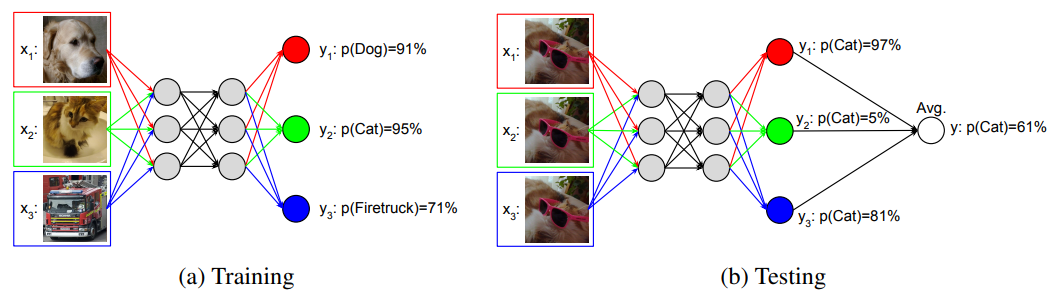
\includegraphics[scale=0.5]
      {Chapter2/Chapter2Figs/mimo.png}    
    \fi
    \caption{Figure Showing the training and testing procedures in MIMO networks}
    \label{mimo}
  \end{center}
\end{figure}

Fig.\ref{mimo} shows the training and testing pipelines for a toy neural network. Number of outputs in a MIMO network need to be equal to the total number of classes like in regular single input multiple output classification networks. But, it needs multiple images as inputs. During training the input images can be different, while during testing, all the input images have to be same.

Results in \cite{havasi2021training} show robustness of the model was improved by ensembling the predictions made by the subnetworks without increasing compute.Particularly, significant improvement in negative log-likelihood, accuracy, and calibration error was observed.

\section{Model Calibration}

Model Calibration is the method of adjusting the predictions made by a trained model to improve their reliability or align them with the desired outcome probabilities. This becomes crucial when using machine learning models in domains where well-calibrated probabilities are essential for informed actions or risk assessments. We don't just want the model to give outputs but also make sure that the model predicts with right amount of confidence. Let's say we have a binary classifier and it predicts an instance with the value 0.6. Although we may interpret it as belonging to class 1, it is important to understand that the model predicted it as class 1 with only 60\% confidence. In a real life medical setting, it is important that the model predictions are neither underconfident nor overconfident. 

\begin{figure}[!htbp]
  \begin{center}
    \leavevmode
    \ifpdf
      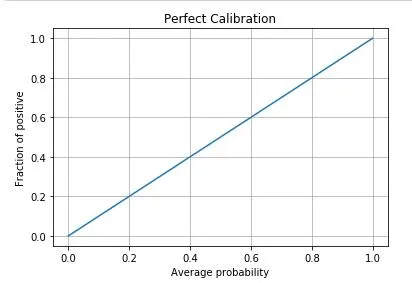
\includegraphics[scale=0.7]
      {Chapter2/Chapter2Figs/per_cal.png}    
    \fi
    \caption{The plot of a perfectly calibrated model}
    \label{per_cal}
  \end{center}
\end{figure}

In order to align the model probabilities with ground truth distribution and predict with appropriate confidence, we calibrate the model outputs. Various methods have been proposed over the years to calibrate the model probabilities like Histogram Binning (\cite{zadrozny2001obtaining}), Isotonic regression (\cite{zadrozny2002transforming}), Bayesian Binning (\cite{naeini2015obtaining}), Platt Scaling (\cite{platt1999probabilistic}) and Temperature scaling (\cite{guo2017calibration}. However, we decided to go ahead with temperature scaling for calibrating the model probabilities due to the promise it showed in calibrating model probabilities of various CNN models such as DenseNet and ResNet when trained on popular datasets like ImageNet and CIFAR-100.

\subsection{Temperature Scaling}

Temperature Scaling is a post-processing technique that was proposed by \cite{guo2017calibration} to improve upon the calibration error by dividing the logits by a learned scalar parameter called Temperature. It is an extension of Platt scaling and uses a single scalar parameter T > 0 for all classes where T is the temperature. Temperature is learned by minimizing the negative log likelihood between model logits divided by temperature and true values. The new softmax function which provides the calibrated probabilities is given as:

\begin{center}
{ $softmax=\frac{e^{z/T}}{\sum_ie^{z_i/T}}$}
\end{center}

When $T>1$, the softmax values is softened, in other words the output entropy is raised. As T → $\infty$, the probability $p_i$ approaches 1/N, which represents maximum uncertainty. With T = 1, we recover the original
probability $p_i$. As T → 0, the probability collapses to a
point mass (i.e. $p_i$ = 1). One more thing to note is that since the parameter T does not change the maximum of the softmax function, the class
prediction does not change on applying Temperature Scaling.

% ------------------------------------------------------------------------

%%% Local Variables: 
%%% mode: latex
%%% TeX-master: "../thesis"
%%% End: 
